\documentclass[11pt]{article}
\usepackage[english]{babel}
\usepackage[a4paper,top=2cm,bottom=2cm,left=3cm,right=3cm,marginparwidth=1.75cm]{geometry}
\usepackage[hyphens]{url}
\usepackage[colorlinks=true, allcolors=blue]{hyperref}
\usepackage{graphicx}
\usepackage{float}

\title{What the Hell is Latex and How Do I Use it}
\author{Helpful Person}
\date{\today}

\begin{document}

\maketitle

\begin{abstract}
   Latex is the standard word-processing tool used for research papers and reports at tertiary institutions. Latex gives the user more control than word processing applications such as Microsoft Word, and can be a powerful tool for formatting reports to your specific needs. 
\end{abstract}

\section{Introduction}
This document was made using Latex and will contain some helpful tips and tricks to get you started using Latex.

\section{How Can I Use Latex}
Head over to \href{https://www.overleaf.com/}{overleaf.com} for a simple way to use latex. Overleaf also allows for collaboration, so multiple people can work on a document at the same time - great for group reports.

\section{Sections and Subsections in Latex}
Latex allows you to use sections and subsections.
\subsection{I am a subsection}
This is a subsection.
\subsubsection{I am a sub-subsection}
Here we are in a sub-subsection.
\section{Figures in Latex}
Let's put a picture in this document:
\begin{figure}[H]
    \centering
    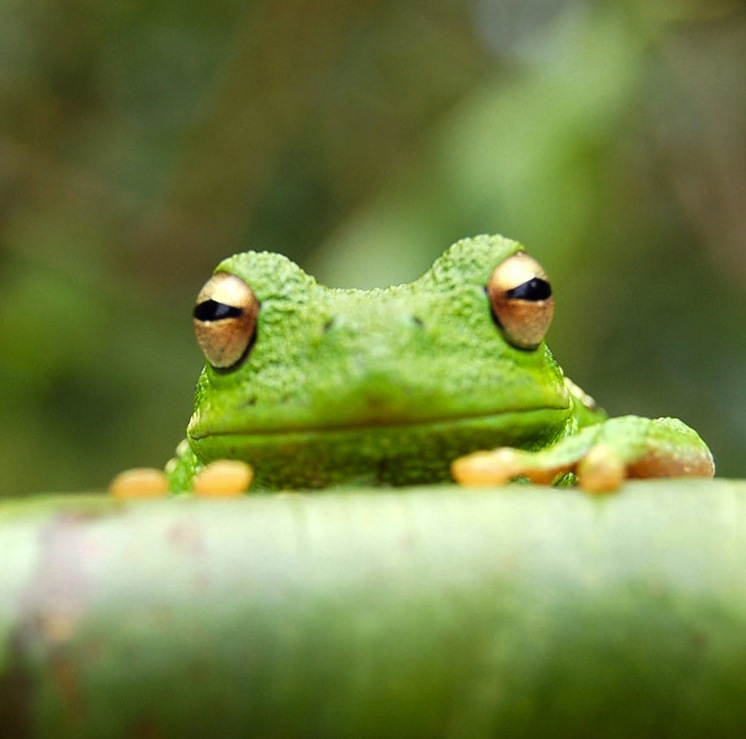
\includegraphics[width=2cm]{frog.jpg}
    \caption{A nice picture of a frog.}
    \label{fig:1}
\end{figure}
Let's make this picture even bigger.
\begin{figure}[H]
    \centering
    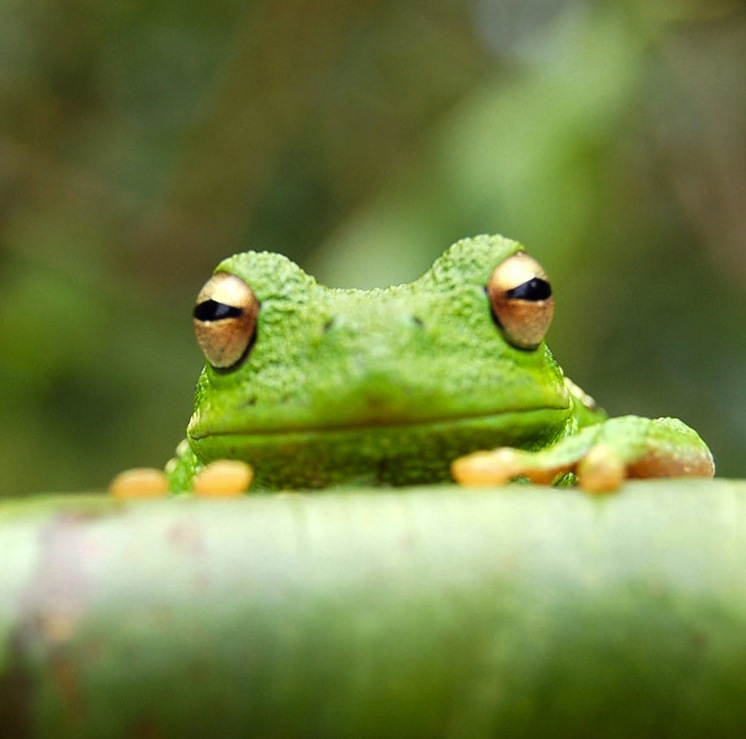
\includegraphics[width=10cm]{frog.jpg}
    \caption{A nice big picture of a frog.}
    \label{fig:2}
\end{figure}
Let's add a figure showing how we did this:
\begin{figure}[H]
    \centering
    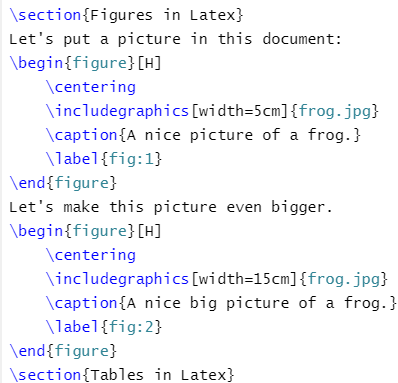
\includegraphics[width=6cm]{screenshot.png}
    \caption{Screenshot of helpful latex code...}
    \label{fig:3}
\end{figure}
Let's break down the code in the above snippet.

\begin{itemize}
  \item First, we begin our figure.
  \item Do you see the little "H" in square brackets? This little guy makes sure that our figures are right where we want them to be in our document, leave it out and latex will push it somewhere else.
  \item We then use centering to make sure our image is nice and centered.
  \item With include graphics, we link the picture that we uploaded to Overleaf. We also set the width of our image in cm.
  \item The caption is where we put the caption of our image.
  \item We use labels so that we can reference our figures elsewhere in the document, like this \ref{fig:1}.
\end{itemize}
\section{Tables in Latex}
Below is a table, made in Latex.
% Table of voltage and current values
\begin{table}[h]
  \centering
  \caption{Voltage and Current Values}
  \begin{tabular}{|c|c|c|}
    \hline
    Component & Voltage (V) & Current (A) \\
    \hline
    Resistor 1 & 5.0 & 0.2 \\
    Resistor 2 & 3.3 & 0.1 \\
    Capacitor 1 & 0.0 & 0.0 \\
    \hline
  \end{tabular}
\end{table}

Making tables in Latex can be tedious. So here's a great tool that you can use instead: \href{https://www.tablesgenerator.com/}{tablesgenerator.com}.

With this website, you can make your tables in a simple program like Excel and then export them into Latex code, which you can easily paste into Latex.

You should take a look at the Latex documentation to find out more about making cool tables in latex.

\section{Maths in Latex}
You can put fun and fancy maths equations in Latex, like so:
\begin{equation}
    f(x) = \frac{1}{x^2 + 2x + 1}
\end{equation}

\begin{equation}
    e^{i\pi} + 1 = 0
\end{equation}

\begin{equation}
    \int_{0}^{\infty} e^{-x^2} \, dx = \frac{\sqrt{\pi}}{2}
\end{equation}

\begin{equation}
    \sum_{n=1}^{100} n = \frac{100 \times 101}{2}
\end{equation}

\begin{equation}
    \lim_{x \to 0} \frac{\sin(x)}{x} = 1
\end{equation}

Here is an image showing you the latex code for these equations:
\begin{figure}[H]
    \centering
    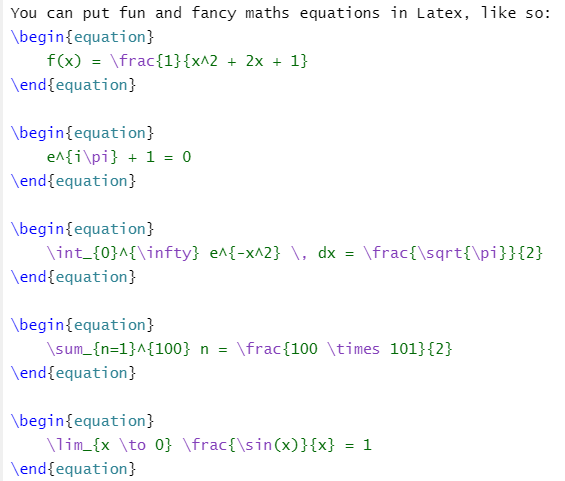
\includegraphics[width=6cm]{screenshot2.png}
    \caption{Screenshot of latex code showing how to make equations.}
    \label{fig:4}
\end{figure}
\section{Referencing in latex}
Let's say you are required to have a list of figures and tables in your document, Latex lets you do this:
\listoffigures
\listoftables

Now I'm doing some research on penguins. Penguin fact number one, they're so cute \cite{davis2012penguinspecies}. Here's another fact, they can't fly \cite{smith2008penguins}. And here's one more fact, I love them \cite{wwf2020penguinconservation}.

Want to know how I did those great citations? Here is a screenshot:
\begin{figure}[H]
    \centering
    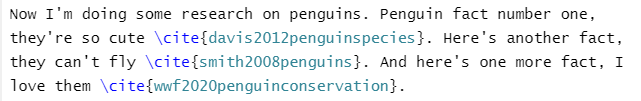
\includegraphics[width=15cm]{screenshot3.png}
    \caption{Citations in latex.}
    \label{fig:5}
\end{figure}

How do we make sure that our citations show up as our references? We simply do the following:

\begin{figure}[H]
    \centering
    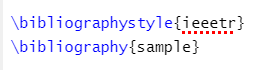
\includegraphics[width=15cm]{screenshot5.png}
    \caption{Referencing my bibliography in latex..}
    \label{fig:6}
\end{figure}


And what does my bibliography look like?

\begin{figure}[H]
    \centering
    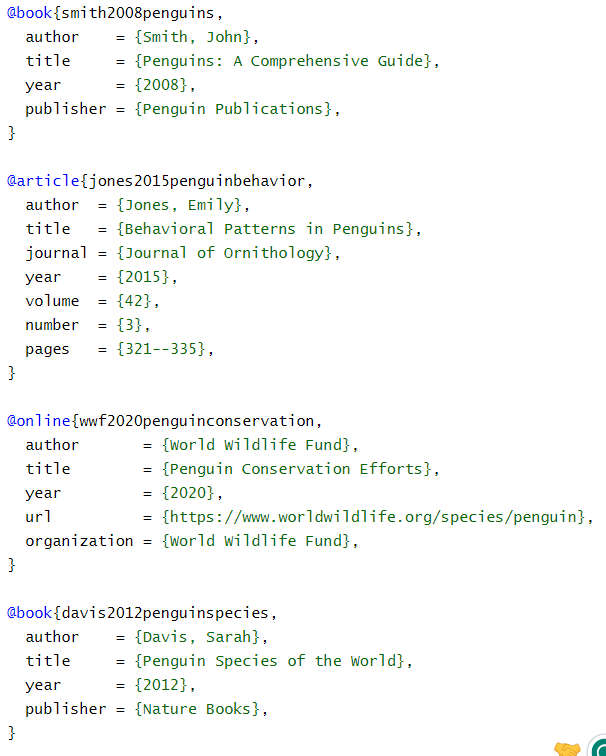
\includegraphics[width=10cm]{screenshot4.png}
    \caption{A latex bibliography.}
    \label{fig:7}
\end{figure}

In Overleaf my bibliography file is called sample.bib. That is where the references are placed and then subsequently referenced by Latex. Below you can see what the file structure for this document looks like in Overleaf.
\begin{figure}[H]
    \centering
    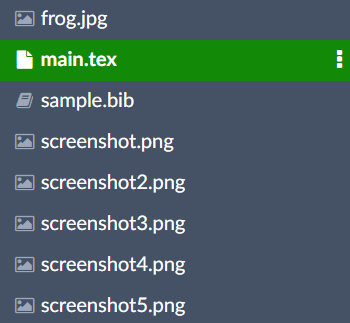
\includegraphics[width=10cm]{screenshot6.png}
    \caption{Overleaf file structure.}
    \label{fig:8}
\end{figure}

\section{Conclusion}
Now you basically know how to use Latex! There is so much more you can find out by reading the Latex documentation, which is very extensive and helpful. ChatGPT can also be your friend!

You can also find the Latex file that this document uses here: 

\bibliographystyle{ieeetr}
\bibliography{sample}

\end{document}
